\documentclass{article}

\usepackage[utf8]{inputenc}
\usepackage{foar705journal}
\usepackage{subfiles}
\usepackage{minted}
\usepackage{ifthen}
%https://tex.stackexchange.com/questions/170739/fancyverb-error-when-using-minted-in-a-ifthenelse
\usepackage{graphicx}
\usepackage{enumitem}

\graphicspath{{./Figures/}}

\newboolean{printCode}
\setboolean{printCode}{true}
%https://tex.stackexchange.com/questions/170739/fancyverb-error-when-using-minted-in-a-ifthenelse

\newcommand{\startdeflist}[0]
{\begin{description}[style=unboxed, labelwidth=\linewidth,
font =\sffamily\itshape\bfseries, listparindent =0pt,
before =\sffamily]}

\title{Learning Journal Weeks 9 - 13}
\author{Bree Kelly}
\date{}

\begin{document}

\maketitle

\tablesofcontentsanderrors

\newpage
\section{Tuesday October 15th 2019}

\subsection{Data Carpentry}
\textbf{Intention:} Complete Data Carpentry on R, lessons 3 and 4.

\textbf{Actions:} Following the instructions on the Data Carpentry website, I go through the lessons and answer the following questions:

\subsubsection{Lesson 3: Starting with Data}

\textit{What is a data.frame?}

The representation of data in the format of a table where the columns are vectors that all have the same length. It is a data structure that forms a building template for data. It does the same thing every time. Infrastructure for data.

\textit{How can I read a complete csv file into R?}

Run the function \mintinline{R}|read_csv(filename)|. 

You can also use the function view to see it in the top left pane.

\textit{How can I get basic summary information about my dataset?}

Using functions such as \mintinline{R}|dim()| (no. of rows and columns), \mintinline{R}|nrow()| (no. of rows), \mintinline{R}|ncol()| (no. of columns), \mintinline{R}|head()| (shows first 6 rows), \mintinline{R}|tail()| (shows last 6 rows), \mintinline{R}|names()| (shows column names), \mintinline{R}|str()| (structure of object), and finally \mintinline{R}|summary()| (returns summarised statistics for each column).

\textit{How do I convert between strings and factors?}

Using \mintinline{R}|factor()|

\textit{Describe the difference between a factor and a string.}

Im not sure about this one.

\textit{Why would I want strings to be treated differently?}

Depends on the type of data analysis you wish to employ and how you what to extract information.

\textit{How do I reorder and rename factors?}

By specifying the factor you wish to rename using \mintinline{R}|[]| with an integer inside and assigning (using an arrow) the new name. To reorder them, you use the assign function, combine function and factor function, eg.

\ifprintCode
%https://tex.stackexchange.com/questions/170739/fancyverb-error-when-using-minted-in-a-ifthenelse
\begin{minted}[breaklines]{R}
memb_assoc <- factor(memb_assoc, levels = c("No", "Yes", "Undetermined"))
\end{minted}
\fi
%https://tex.stackexchange.com/questions/170739/fancyverb-error-when-using-minted-in-a-ifthenelse

\textit{How do I change how character strings are handled in a data frame?}

Turn them into numerical integers, eg, \mintinline{R}|as.numeric(as.character(year\_fct))|

\itemizederror{No package called Tidyverse}{
\item I started by downloading R and RStudio onto my laptop, then switching to my Surface, on which the CSV file of cleaned SAFI data that I produced in the OpenRefine Data Carpentry Lessons is located.
\item I followed the instructions to download tidyverse in order to use the \mintinline{R}|read_csv()| function, but running \mintinline{R}|library(tidyverse)| returned `Error in library(tidyverse) : there is no package called ``tidyverse."
\item I swear I already downloaded that package, but okay. I go to the Packages tab and search `tidy. No tidyverse package.
\item I click Install and select tidyverse and set it installing.
\item Installation is a success.}

I run \mintinline{R}|library(tidyverse)| again. It returns this:

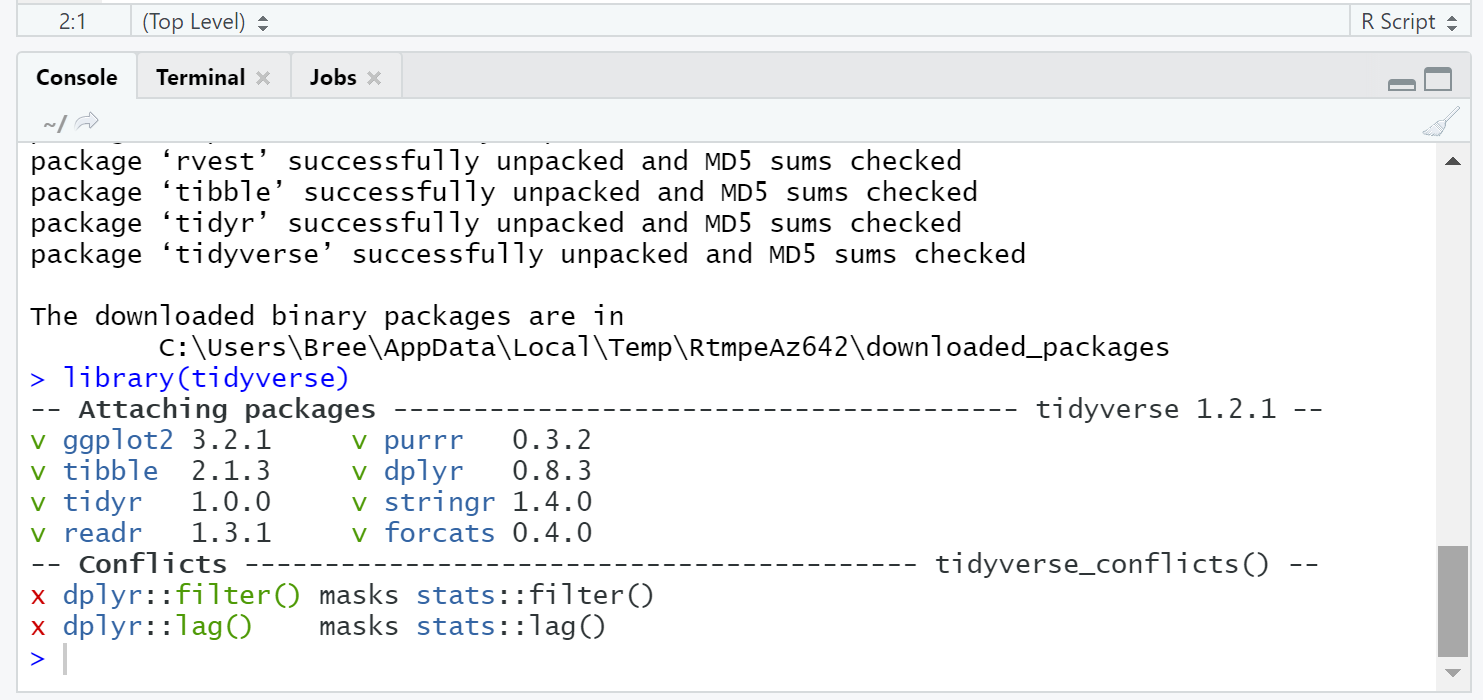
\includegraphics[width=1.0\textwidth]{rstudio_14.PNG}

I copy the CSV file I want to work with (\mintinline{R}|SAFI_clean_exercise_CSV.csv|) into the working directory (Computer/Documents/). I run

\begin{minted}[breaklines]{R}
interviews <- read_csv("SAFI_clean.csv", na = "NULL") 
\end{minted}

 as per the instructions, leaving out the part of the file name I added (ie.\mintinline{R}|_exercise_CSV|) because I am an idiot. Of course, this is returned: Error: unexpected `NULL in
 
\begin{minted}[breaklines]{R}
interviews <- read_cscv("SAFI_clean.csv, na = "NULL")
\end{minted}
 
 I now notice I left out the double quotation mark at the end of the file name, so I correct this, and it finally prints the following:

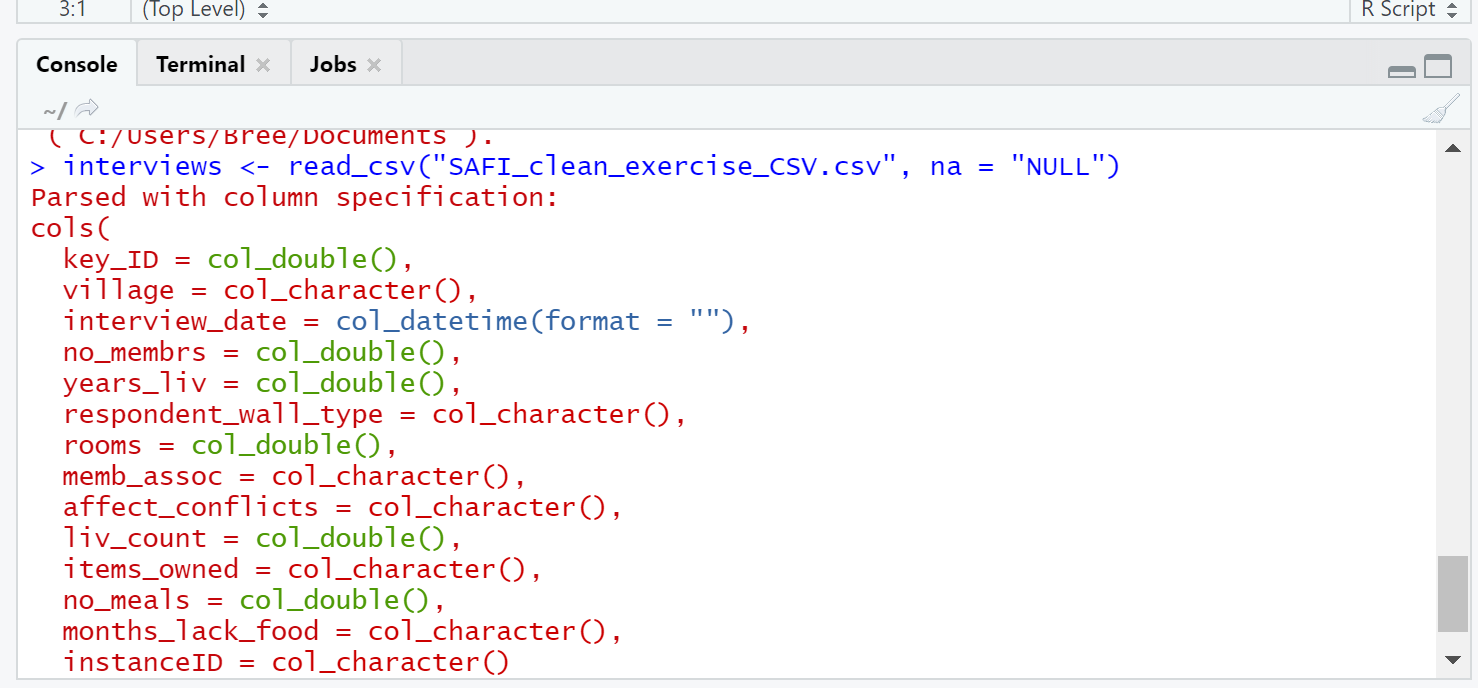
\includegraphics[width=1.0\textwidth]{rstudio_15.PNG}

I can finally move on. I try running just `interviews to see the file:

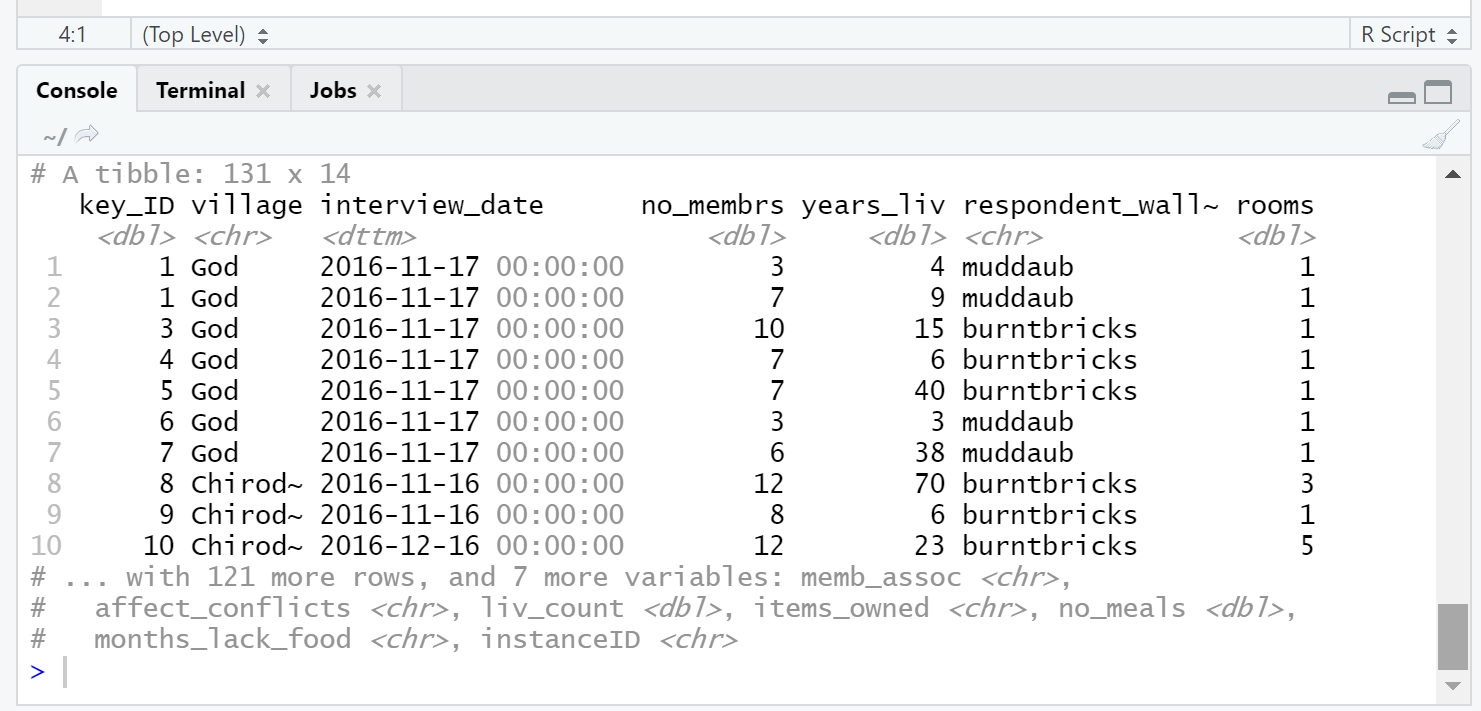
\includegraphics[width=1.0\textwidth]{rstudio_16.PNG}

I then try \mintinline{R}|view(interviews)|, which returns an excel-sheet-looking table in a new tab within the top left pane:

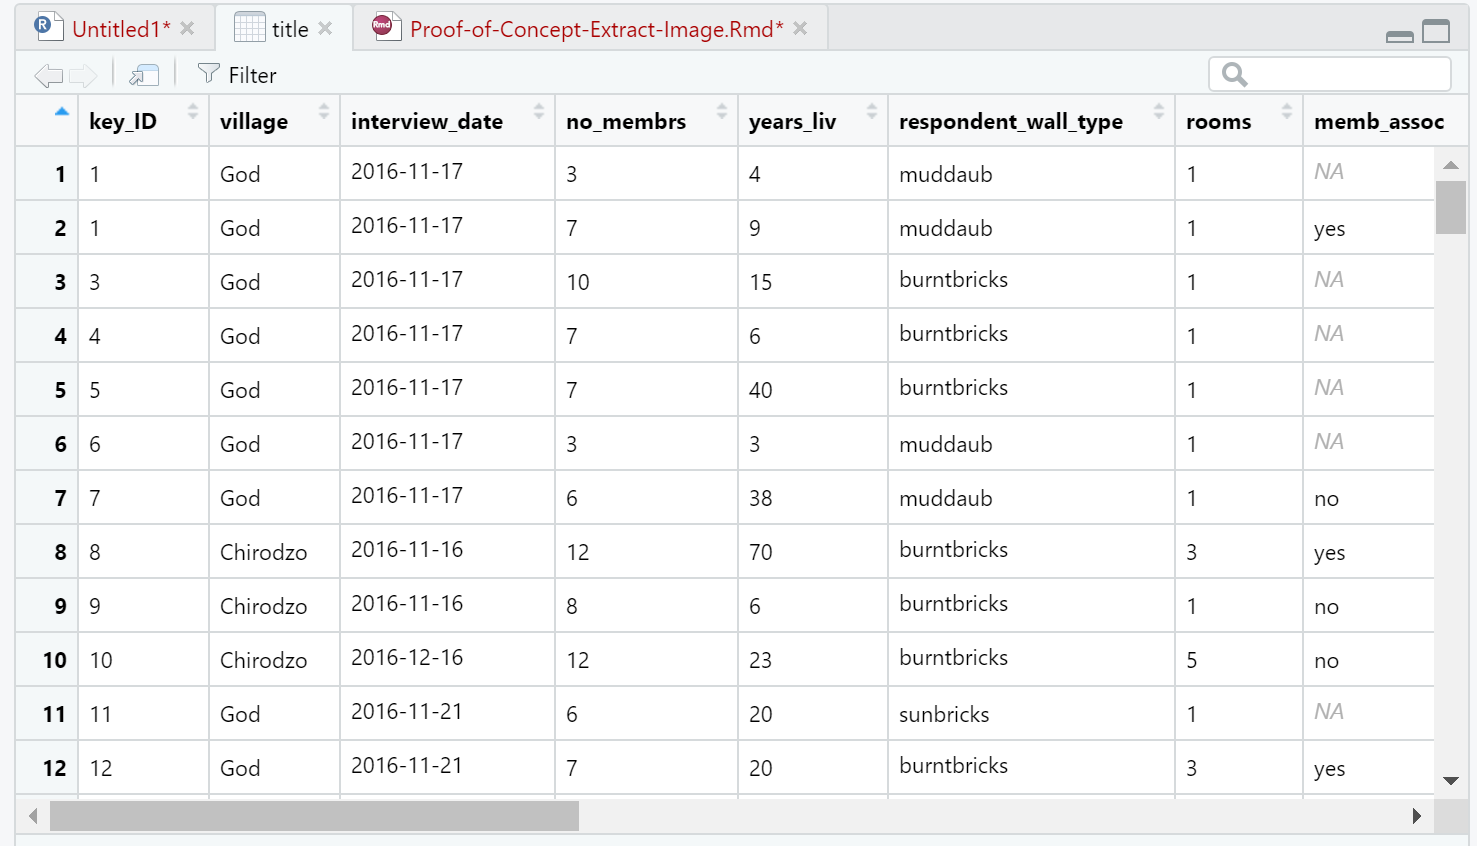
\includegraphics[width=1.0\textwidth]{rstudio_17.PNG}

I then try \mintinline{R}|head(interviews)|, which returns this:

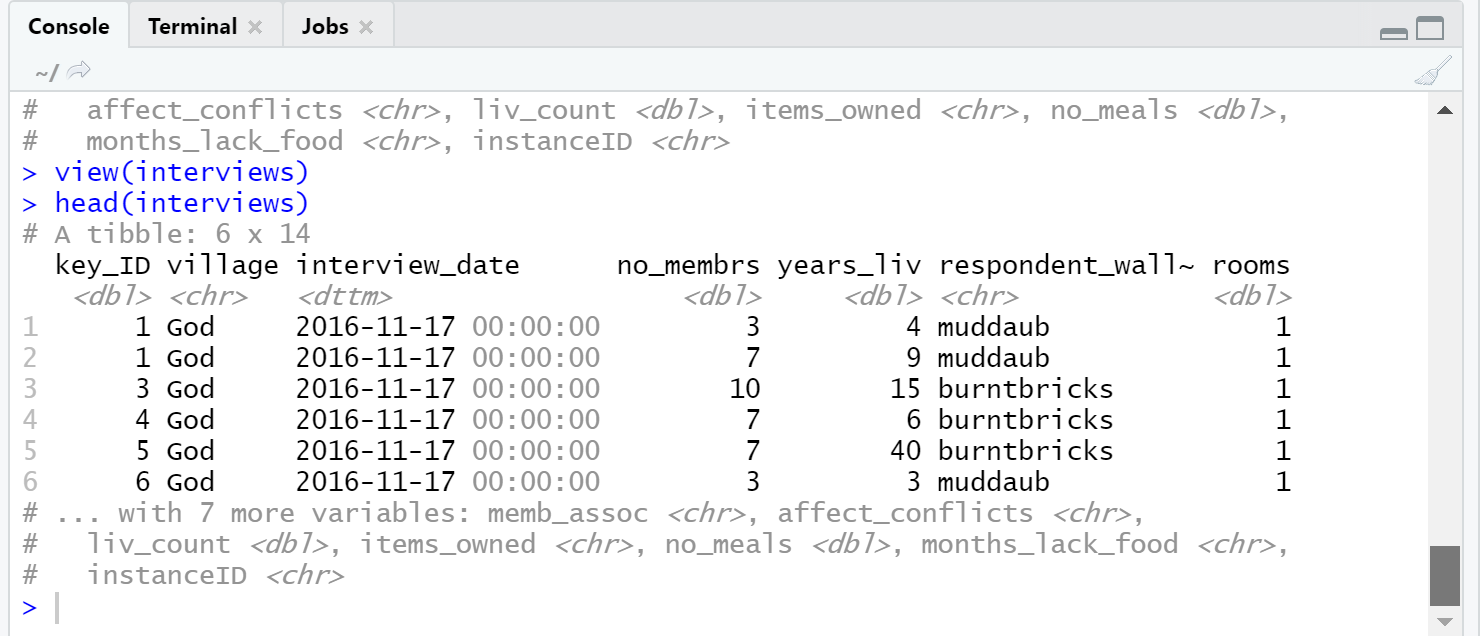
\includegraphics[width=1.0\textwidth]{rstudio_18.PNG}


\itemizederror{Missing Variable?}
{\item (refer to previous section and above images)
\item Not sure how to interpret it, but I didnt get an error for once.
\item I read further into the lesson that \mintinline{R}|head(interviews)| prints the first 6 lines of the file, which appears to be the case when I ran it.
\item I run the various ways to specify columns and rows and such, including \mintinline{R}|interviews[1, 1]|, \mintinline{R}|interviews[1, 6]|, \mintinline{R}|interviews[[1]]|, \mintinline{R}|interviews[1]|, \mintinline{R}|interviews[1:3, 7]|, and \mintinline{R}|interviews[3, ]|.
\item They all run fine, except with the last one, although it executes fine, I can see one difference in the results – instead of \mintinline{R}|8 more variables|, mine states that there are \mintinline{R}|7 more variables|, and appears to be missing the \mintinline{R}|rooms <dbl>|.
\item I can also see a 1 after \mintinline{R}|burntbricks| on my console, which does not appear in the example.
\item Maybe rooms is over there somewhere. I cant figure it out.}

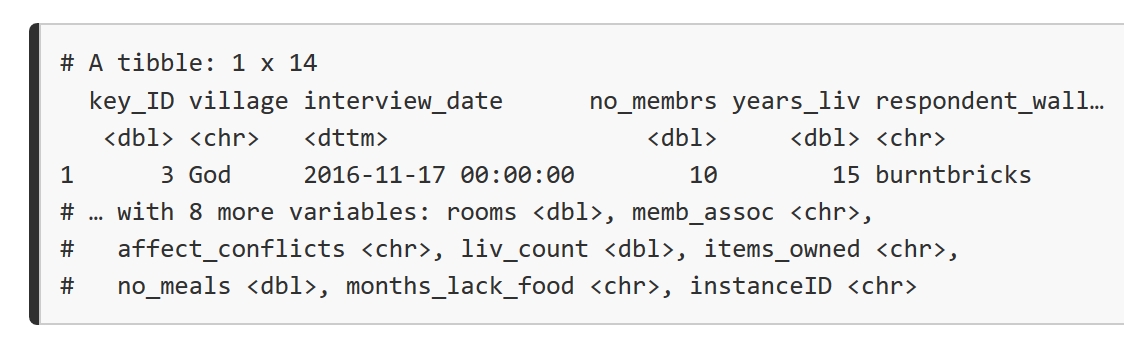
\includegraphics[width=1.0\textwidth]{rstudio_19.PNG}

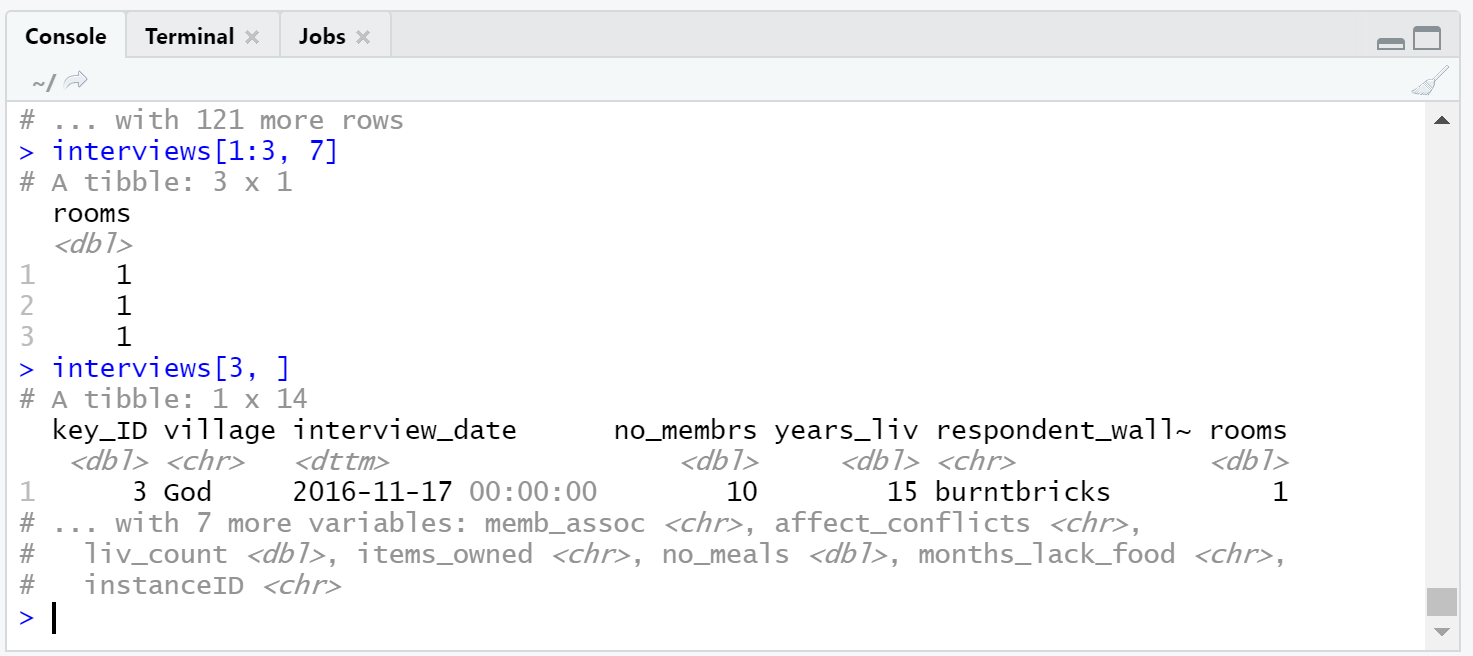
\includegraphics[width=1.0\textwidth]{rstudio_20.PNG}

I tried to complete the following exercise:

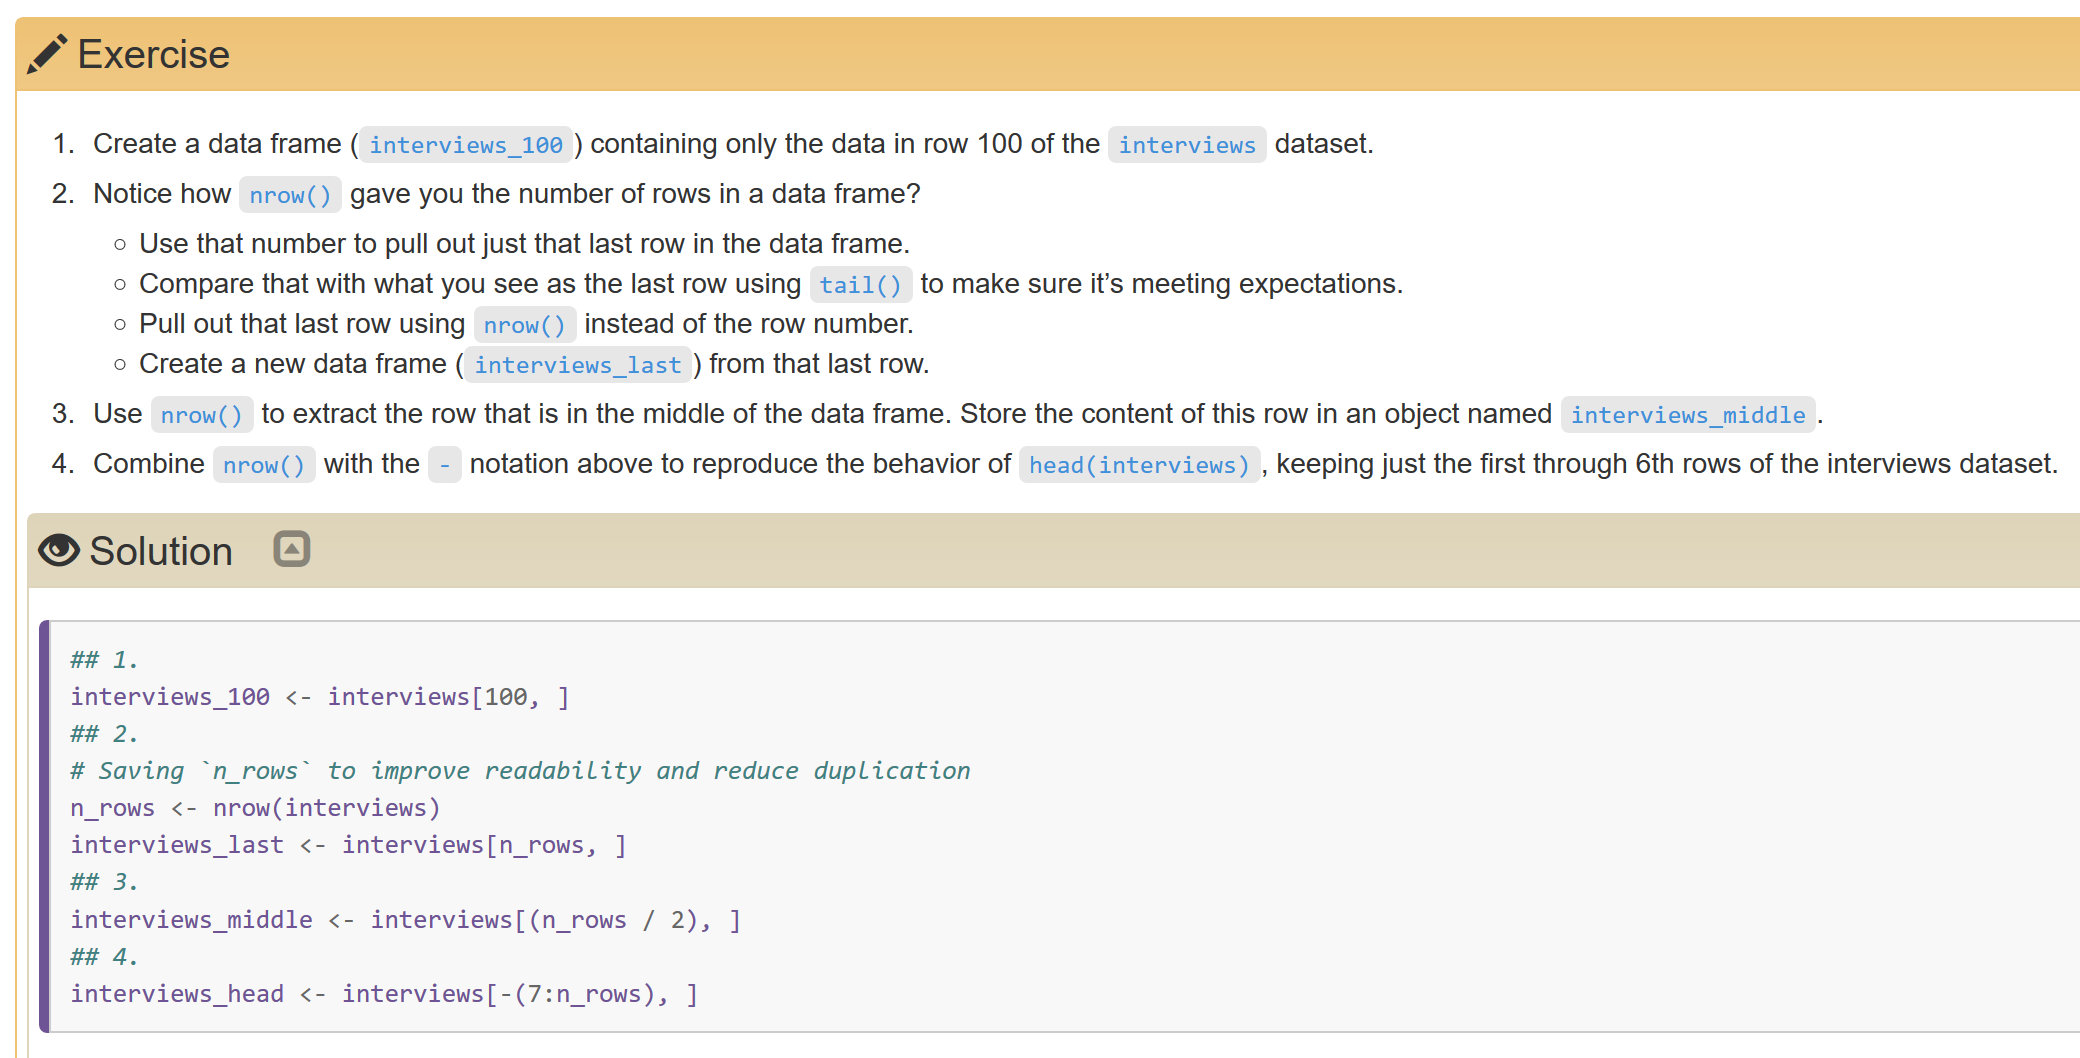
\includegraphics[width=1.0\textwidth]{rstudio_21.PNG}

I did the first part correctly (\mintinline{R}|interviews <- interviews[100, ]|), but got stuck after that. I feel like the instructions are not clear. The second part sounds like its using what you created in the first part, but maybe thats not the case. I tried a few different things, but had to look at the Solution, and even then, I cant fully grasp what is happening in the exercise. I need more help and explanation on this one. Going through the lesson a second time, I think I understand it a little better, but Im still not 100 per cent on vectors, strings, and factors.

\textbf{Result:} Lesson 3 completed (to best of my ability) and recorded in Learning Journal.

\section{Wednesday October 23rd 2019}

\subsection{Data Carpentry}

\subsubsection{Lesson 4: Introducing \mintinline{R}|dplyr| and \mintinline{R}|tidyr|}

\textbf{Intention}: Complete Data Carpentry on R, Lesson 4.

\textbf{Action}: Following the instructions on the Data Carpentry website, I go through the lessons and answer the following questions:

\textit{How can I select specific rows and/or columns from a data frame?}

Select(data frame, column name, column name, column name)

`To select columns of a data frame, use \mintinline{R}|select()|.

The first argument to this function is the data frame (\mintinline{R}|interviews|), and the subsequent arguments are the columns to keep.

To be more specific, use \mintinline{R}|filter|:

\mintinline{R}|filter(data frame, column name == "column component")|

\textit{How can I combine multiple commands into a single command?}

There are three ways to combine commands.
Intermediate steps, nesting, and pipes.
Intermediate steps works, but is messy.
Nesting is ‘neater,’ but can become difficult to keep track of things.
Pipes is the preferred method.

Exercise – my answer: 

\begin{minted}[breaklines]{R}
interviews_members <- interviews%>%
filter(memb_assoc == "yes")%>%
select(affect_conflicts, liv_count, no_meals)
\end{minted}

Checking solution, I see that I got this down pat.

\itemizederror{Understanding Filter Function}
{\item
\begin{minted}[breaklines]{R}interviews_god <- select(filter(interviews, village == "God"), no\_membrs, years\_liv)\end{minted}
\item I don’t understand the break down of this construction.
\item \mintinline{R}|filter| acts on \mintinline{R}|interviews| as the data frame, but what data frame does \mintinline{R}|select work| on in order to also select \mintinline{R}|no_members| and \mintinline{R}|years_liv?|}
\textit{How can I create new columns or remove existing columns from a data frame}?
Using the \mintinline{R}|mutate| function, you can add a column by using information in other columns.
In the exercise, I got an answer that was close, but in the wrong order:
\begin{minted}[breaklines]{R}
interviews_village <- interviews%>%
select(village)%>%
mutate(total_meals = no_members*no_meals)%>%
select(total_meal > 20)
The correct answer was:
interviews_village <- interviews%>%
mutate(total_meals = no_membrs * no_meals)%>%
filter(total_meal > 20)%>%
select(village, total_meals)
\end{minted}
I realised after trying it out that it should be \mintinline{R}|no_membrs|, not \mintinline{R}|no_members|, and I made a typo when writing \mintinline{R}|total_meals| (I left off the s).
After fixing these small issues, it worked fine.
\textit{How can I reformat a dataframe to meet my needs}?
Eeshaping by gathering and spreading – creating new tables using variables and values within the original data frame.
\itemizederror{Mismatch between Data Carpentry and RStudio}
{\item When completing the exercise for this, I copied the instructions directly into RStudio, and I couldn’t see the correlation between what I was seeing in RStudio and on the Data Carpentry website.
\item It indicated that a separate new table would be created with 4 rows, but it appeared to just add them onto the end of the existing table:
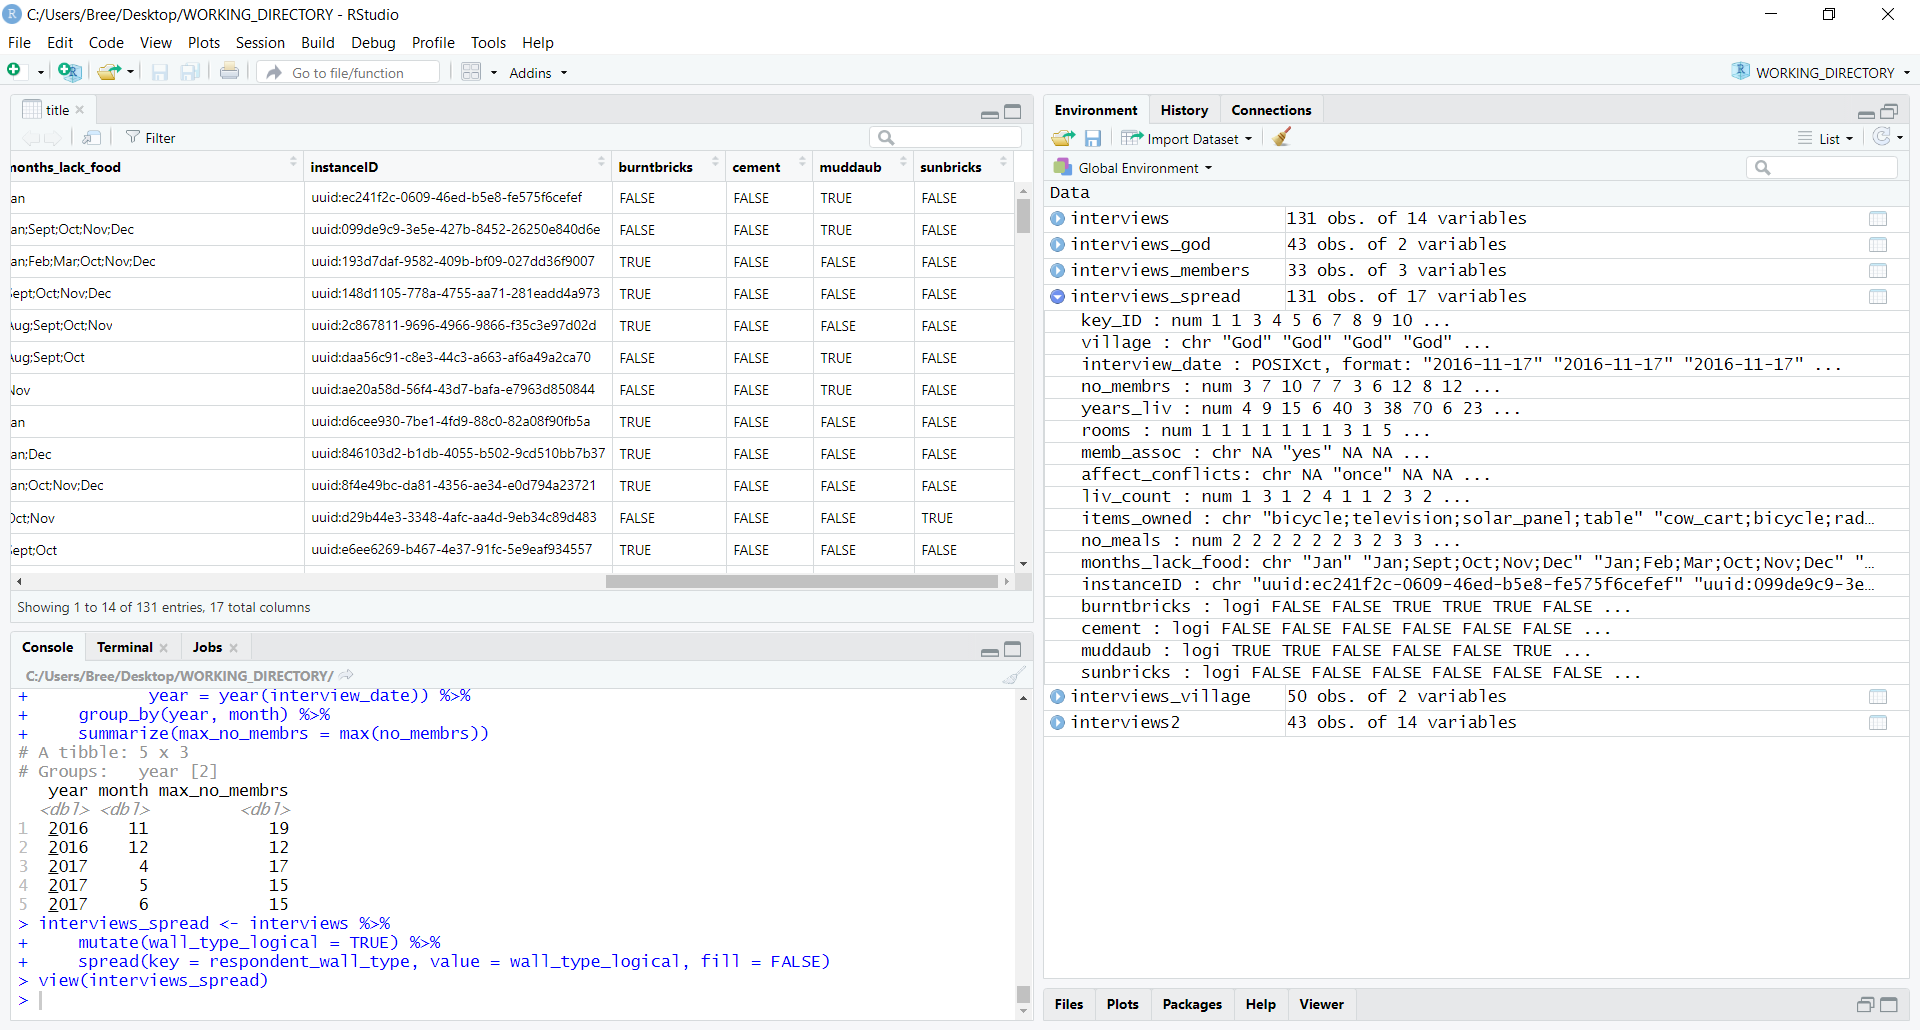
\includegraphics[width=1.0\textwidth]{rstudio_22.PNG}
This seems to be how it’s supposed to work, but I’m not fully wrapping my head around the concept. The highlighted line is the one I’m having trouble understanding:
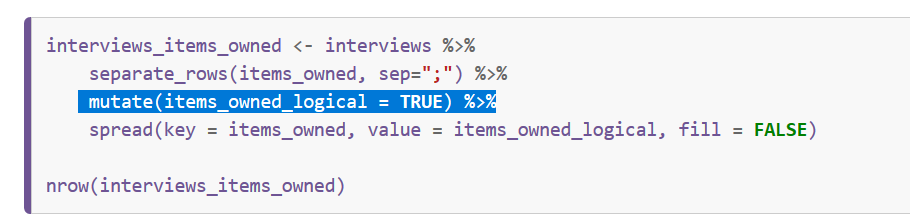
\includegraphics[width=1.0\textwidth]{rstudio_23.PNG}}

\itemizederror{??}
{\item The exercise going through the Applying \mintinline{R}|spread()| to clean our data process states that the last column in the data frame after running 
\begin{minted}[breaklines]{R}
interviews_items_owned <- interviews \begin{verbatim}%>%\end{verbatim}
separate_rows(items_owned, sep=";") \begin{verbatim}%>%\end{verbatim}
mutate(items_owned_logical = TRUE) \begin{verbatim}%>%\end{verbatim}
spread(key = items_owned, value = items_owned_logical, fill = FALSE)’
\end{minted}
is \begin{verbatim}/end{verbatim} and that it needs to be renamed to be called `NA, but mine is already called that:
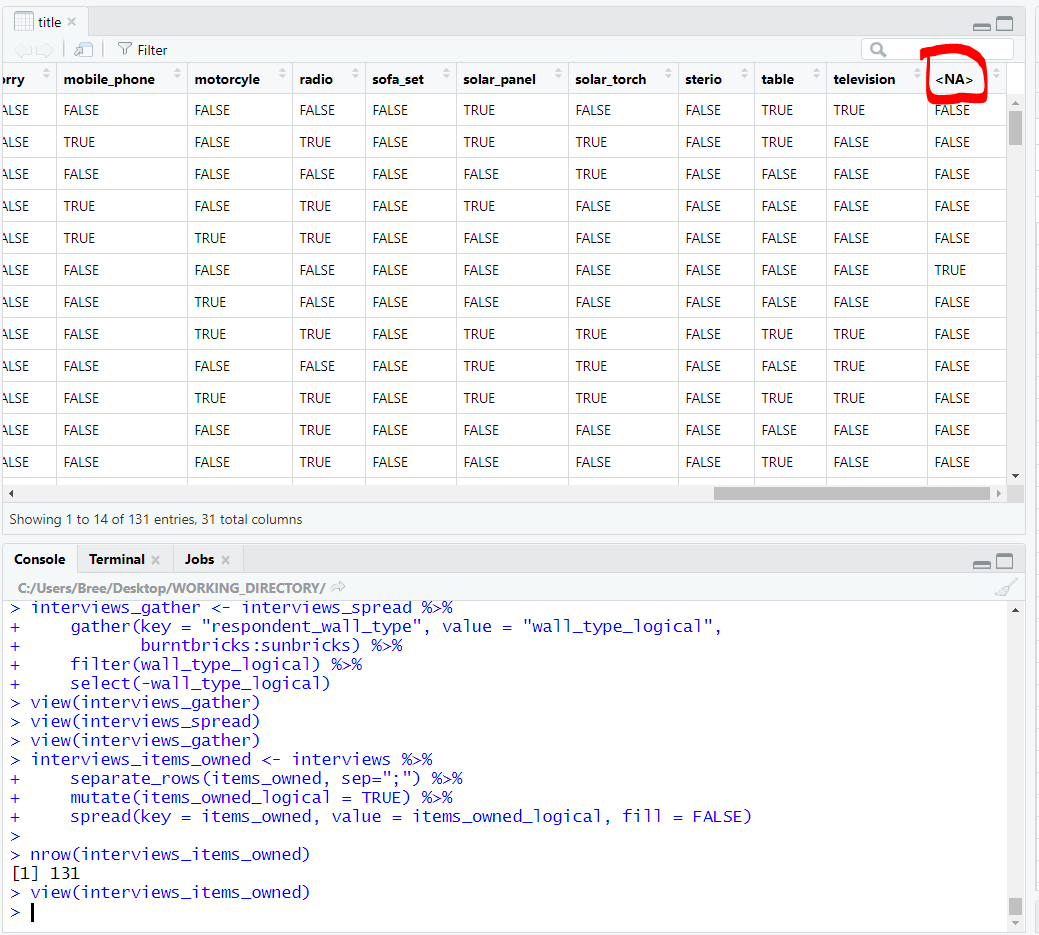
\includegraphics[width=1.0\textwidth]{rstudio_24.PNG}
Reading further on, after running
\begin{minted}[breaklines]{R}
interviews_items_owned <- interviews_items_owned\begin{verbatim}%>%\end{verbatim}
rename(no_listed_items = <NA>)
\end{minted}
to rename the column, I see it has replaced the NA with \mintinline{R}|no_listed_items|.
Perhaps it was just showing NA before because the value was NA, and the Data Carpentry site just expected the value of NA to be shown as \begin{verbatim}/\end{verbatim}.}
\itemizederror{Lack of Explanation}
{\item We haven’t really got an explanation for the \mintinline{R}|rowSums| function and the `. in the following argument:
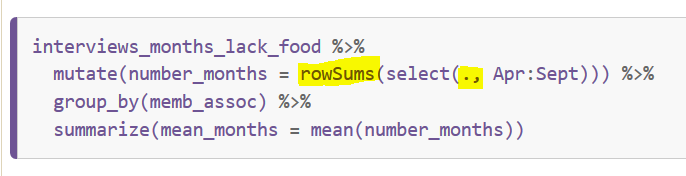
\includegraphics[width=1.0\textwidth]{rstudio_25.PNG}
\item I wrote the final data frame to a csv file then opened the file in Excel to inspect it. \item Success.}
\textbf{Result}: Lesson 4 is complete, and questions are prepared for consultation hour. Next task: complete ‘Lesson 5: Data Visualisation with ggplot2.’

\end{document}